\documentclass[11pt,a4paper]{article}

\usepackage[utf8]{inputenc}
\usepackage[T1]{fontenc}
\usepackage{lmodern}
\usepackage[french]{babel}
\usepackage[margin=2.4cm]{geometry}
\usepackage{microtype}
\usepackage{booktabs}
\usepackage{array}
\usepackage[table]{xcolor}
\usepackage{colortbl}
\usepackage{amsmath}
\usepackage{amssymb}
\usepackage{mathtools}
\usepackage{enumitem}
\usepackage{graphicx}
\usepackage{caption}
\usepackage[most]{tcolorbox}
\usepackage{hyperref}

\definecolor{navy}{HTML}{1F3864}
\definecolor{bluemid}{HTML}{2E5496}
\definecolor{lightblue}{HTML}{D6E0F0}
\definecolor{softgrey}{HTML}{F2F2F2}
\definecolor{accent}{HTML}{C0491F}

\hypersetup{colorlinks=true, linkcolor=bluemid, urlcolor=bluemid,
  pdftitle={Fiche pedagogique - Modele qualitatif de cascade DORA},
  pdfauthor={Kelian Kaddouri}}

\captionsetup{font=small,labelfont={bf,color=navy},labelsep=period}

\newcommand{\chaine}[1]{\ensuremath{#1}}
\newcommand{\fl}{\ensuremath{\!\rightarrow\!}}

\newtcolorbox{cle}[1][]{colback=lightblue!40,colframe=navy,boxrule=0.6pt,
  arc=2pt,left=8pt,right=8pt,top=6pt,bottom=6pt,#1}

\title{\vspace{-1.2cm}\color{navy}\bfseries Fiche pédagogique\\[2pt]
  \large Comment sont construits les scores du modèle qualitatif de cascade DORA}
\author{Kélian Kaddouri}
\date{\today}

\begin{document}
\maketitle
\vspace{-0.6cm}

\begin{cle}
\textbf{Idée centrale.} On n'évalue pas un \emph{ensemble} de piliers DORA, mais une
\emph{chaîne ordonnée} d'effondrement. Une cascade qui suit une direction causale
plausible (amont~\fl~aval, gouvernance~\fl~conséquences) est un vrai emballement
systémique : plus \textbf{probable} \emph{et} plus \textbf{grave}. Le même ensemble pris
à l'envers est rare et peu grave. \textbf{L'ordre pilote donc le verdict.}
\end{cle}

\section{Les cinq piliers et les trois tables de jugement}

Les cinq piliers de DORA (Règlement UE 2022/2554~\cite{DORA2022}) sont indexés de 1 à 5 :
P1~gouvernance \& gestion du risque TIC ; P2~gestion des incidents ; P3~tests de
résilience (TLPT) ; P4~gestion du risque lié aux tiers ; P5~partage d'informations.

Tout le modèle repose sur \textbf{trois barèmes d'expert}~\cite{Cooke1991,OHagan2006}, et
rien d'autre. Aucune valeur n'est mesurée : ce sont des jugements \emph{ordonnés}, dont
seule la \textbf{hiérarchie} est défendable --- une matrice de risque ne doit jamais être
lue plus finement que son ordre~\cite{Cox2008} (la sensibilité, \S\,\ref{sec:sensi}, montre
que les décimales exactes importent peu). Le principe même d'un score
\emph{criticité $=$ f(probabilité, gravité)} est celui des référentiels de gestion des
risques~\cite{ISO31000,ISO27005}.

\begin{table}[h]\centering\small
\renewcommand{\arraystretch}{1.25}
\begin{tabular}{@{}p{2.1cm} p{5.3cm} p{6.9cm}@{}}
\toprule
\textbf{Table} & \textbf{Rôle} & \textbf{Ancrage logique + DORA} \\
\midrule
$\text{ROOT}[p]$ & Propension du pilier $p$ à \emph{amorcer} une cascade.
  & P1$=1{,}0$ (fondation gouvernance, responsabilité de l'organe de direction, chap.~II) ;
    P4$=0{,}9$ (surface d'attaque externe, cloud) ; P5$=0{,}3$ (rarement déclencheur). \\
$\text{TRANS}[a][b]$ & Force dirigée \og{}$a$ entraîne $b$\fg{}, \textbf{asymétrique}.
  & P1$\fl$tout fort ; tout$\fl$P1 faible ; P4$\fl$P2$=0{,}8$. C'est l'asymétrie qui fait
    que l'ordre compte. \\
$\text{GBASE}[p]$ & Gravité intrinsèque du pilier s'il tombe seul.
  & P4$=7$ : \textbf{contagion systémique} (cadre de supervision des tiers critiques) ;
    P1$=6$ (fondation) ; P5$=1$ : partage \textbf{volontaire} (art.~45) $\Rightarrow$ le
    moins critique. \\
\bottomrule
\end{tabular}
\caption{Les seuls chiffres d'entrée du modèle et leur justification.}
\end{table}

\begin{cle}
\textbf{D'où viennent ces trois barèmes ?} Les \emph{valeurs} sont un jugement d'expert ancré
sur la structure de DORA. Les \emph{concepts}, eux, sont trois primitives standard de
l'analyse de risque, ici recombinées :
\begin{itemize}[leftmargin=1.4em,itemsep=1pt,topsep=2pt]
\item \textbf{ROOT} instancie l'\emph{événement initiateur} de l'analyse probabiliste de
  risque et le \emph{n\oe{}ud-graine} des modèles de cascade, dont l'influence se mesure par la
  taille attendue de la propagation~\cite{KaplanGarrick1981,Kempe2003}.
\item \textbf{TRANS} est une \emph{matrice d'influence dirigée} : ses entrées sont des forces
  d'entraînement, non des probabilités (les lignes ne somment pas à~1). Normalisée ligne à
  ligne, elle devient le \emph{noyau de transition} d'une chaîne de Markov et rejoint les
  réseaux bayésiens~\cite{Pearl1988}, les probabilités d'activation d'arête des modèles de
  cascade~\cite{Kempe2003} et les matrices d'influence du risque systémique~\cite{Battiston2012}.
\item \textbf{GBASE} est l'axe de \emph{sévérité intrinsèque} par composant : la gravité de
  l'AMDEC~\cite{IEC60812} et le score de base CVSS~\cite{CVSS}.
\end{itemize}
Réunies, ces trois briques sont le \textbf{triplet du risque} de Kaplan \& Garrick~\cite{KaplanGarrick1981} :
\emph{quel scénario (ROOT, TRANS), avec quelle probabilité, pour quelle conséquence (GBASE)}.
\textbf{L'apport propre} de ce modèle n'est aucune de ces briques, mais leur mise en
\emph{dépendance de l'ordre} --- le même ensemble de piliers étant noté différemment selon la
direction de la chaîne.
\end{cle}

\section{Construction des deux dernières colonnes}

\subsection*{Colonne \og{}Probabilité conceptuelle\fg{} (rappel, préalable)}

La probabilité part du pilier amorceur et se dégrade à chaque maillon de la chaîne :
\begin{equation}
p \;=\; \operatorname{round}\!\Big(10 \times \text{ROOT}[\text{départ}]
      \times \!\!\prod_{\text{maillons } a\fl b}\!\! \text{TRANS}[a][b]\Big),
\qquad p \in [1,10].
\end{equation}
Une chaîne longue est mécaniquement plus rare (chaque facteur~$<1$). Ce $p$ est une
\textbf{cotation ordinale} sur $[1,10]$, non une probabilité normalisée : il \emph{classe} les
ordres, comme le recommande Cox~(2008)~\cite{Cox2008} pour une matrice de risque, sans prétendre
se sommer à~1. La normalisation en vraie probabilité conditionnelle est traitée à part.

\paragraph{Lecture récursive (structure d'arbre).} Ce produit n'est pas arbitraire : il a
une structure d'\textbf{arbre}. La probabilité d'un ordre de $n$ piliers se \emph{construit}
à partir de son préfixe de $n-1$ piliers, en multipliant par le seul maillon ajouté :
\begin{equation}
p(a\fl b\fl c) \;=\; \underbrace{\text{ROOT}[a]\times\text{TRANS}[a][b]}_{p(a\fl b)}
  \times\text{TRANS}[b][c]
  \;=\; p(a\fl b)\times\text{TRANS}[b][c].
\end{equation}
On engendre ainsi tous les ordres en insérant le pilier suivant à chaque position,
suivant la récurrence $N_n = n\,N_{n-1}$ (2, 6, 24, 120 ordres pour 5~piliers). La
figure~\ref{fig:arbre} déroule cet arbre sur l'exemple à trois piliers, avec les valeurs
réelles du modèle : partir de P1 (gouvernance) est la seule racine vraiment probable~;
toute branche amorcée en aval retombe au plancher.

\begin{figure}[h]\centering
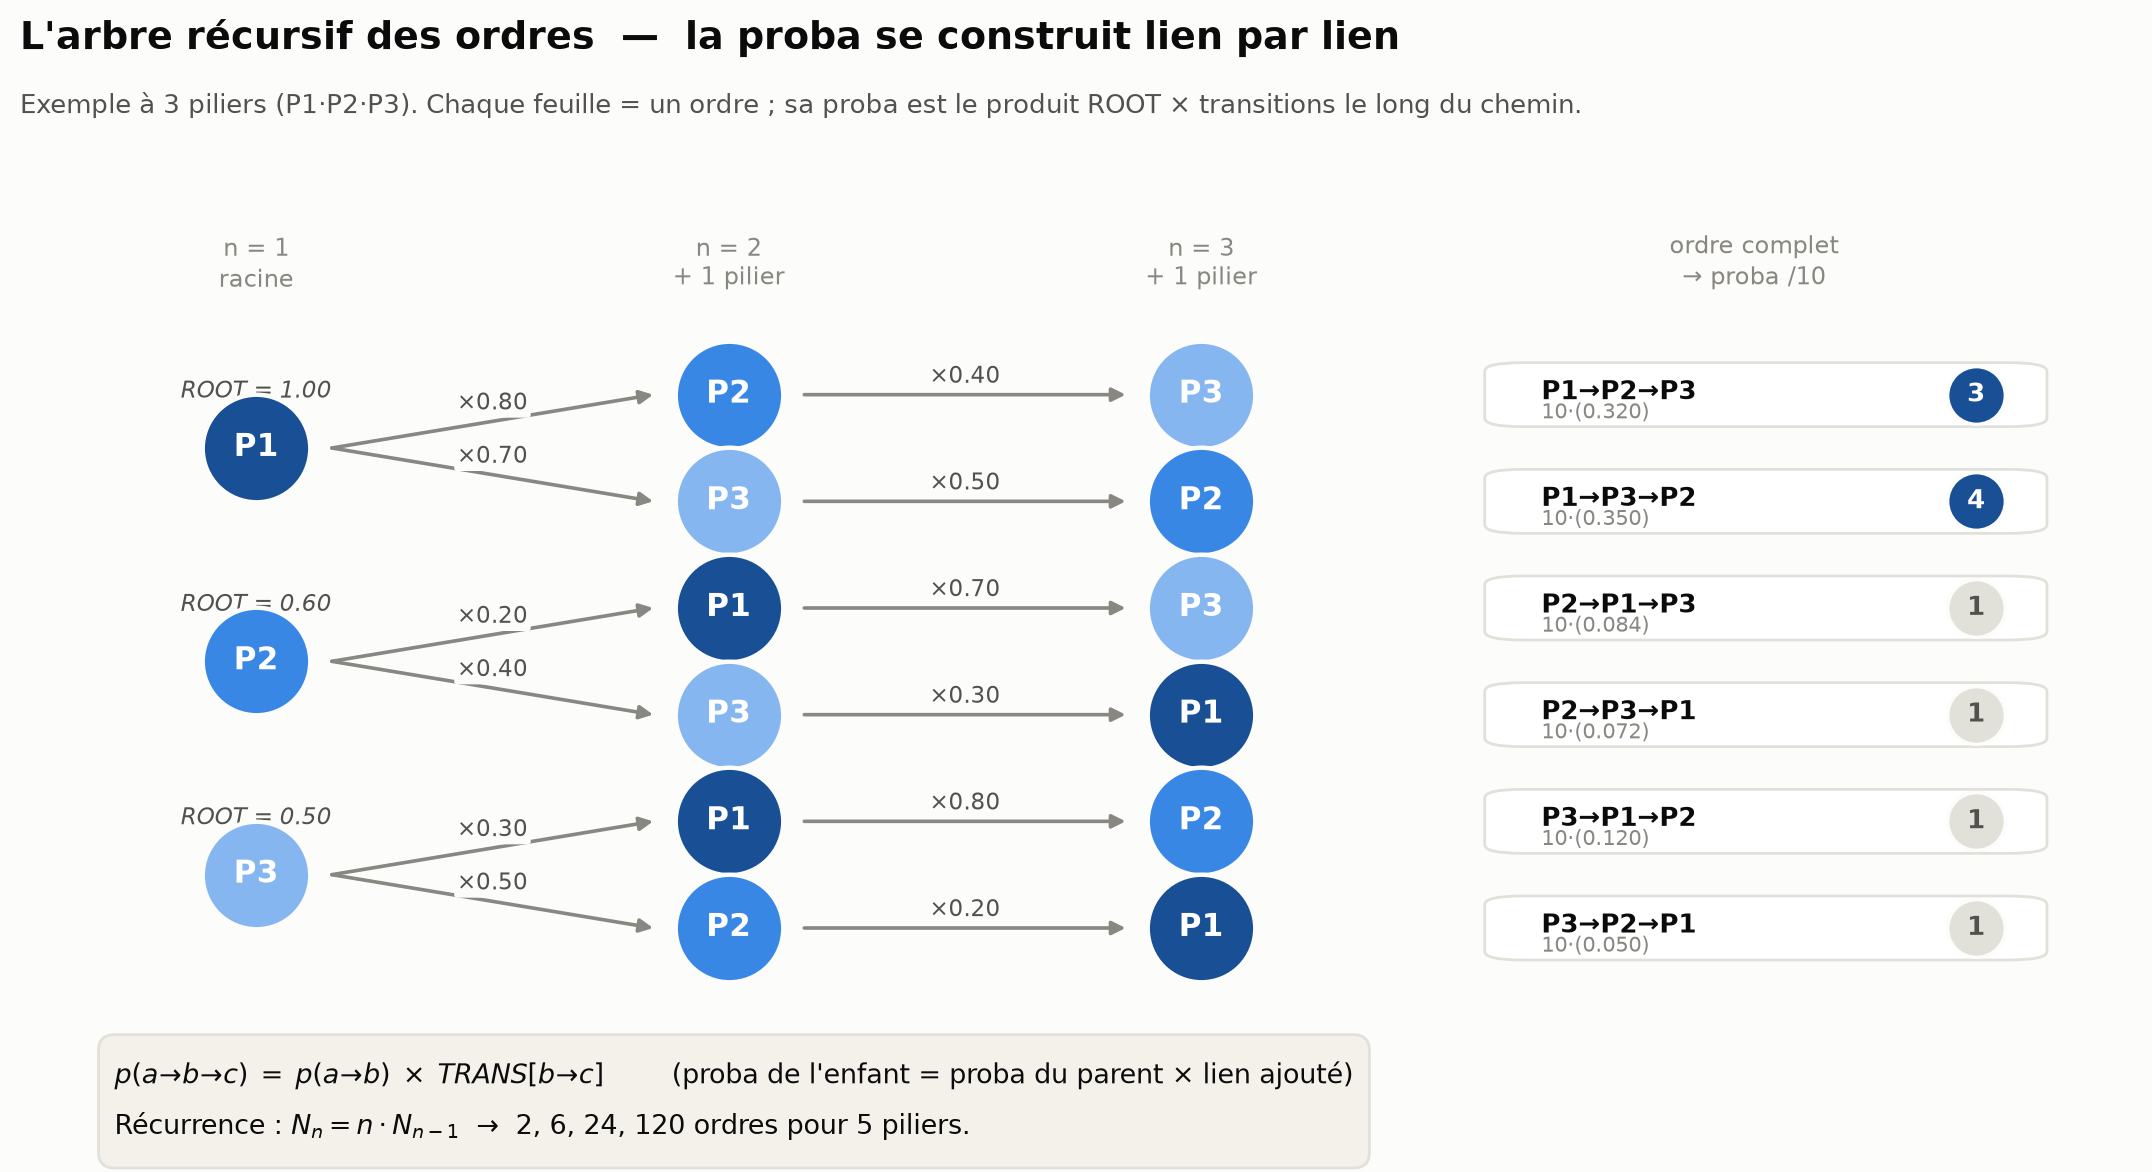
\includegraphics[width=\linewidth]{figures/F12_arbre_recursif.png}
\caption{La probabilité se construit lien par lien le long de l'arbre des ordres :
proba de l'enfant $=$ proba du parent $\times$ transition ajoutée. L'asymétrie de
TRANS (p.\,ex. P1\fl P3 à $0{,}70$ contre P3\fl P1 à $0{,}30$) est ce qui sépare les
verdicts. \emph{N.B.} seule la \textbf{probabilité} se décompose ainsi~; la gravité, elle,
dépend de l'\emph{ensemble} des piliers présents (étendue) et n'est pas multiplicative
le long de l'arbre.}
\label{fig:arbre}
\end{figure}

\subsection*{Colonne \og{}Gravité conceptuelle\fg{}}

La gravité = \emph{étendue des dégâts} \textbf{amplifiée ou amortie} par la cohérence
causale de l'ordre. Elle se lit en trois temps :

\begin{align}
\text{étendue} &= \min\!\Big(10,\; \max(\text{GBASE}) + 0{,}40\times\!\!\sum_{\text{autres piliers}}\!\!\text{GBASE}\Big) \\[2pt]
\text{cohérence} &= \operatorname{moyenne}\big(\text{TRANS}[\text{maillons}]\big) \in [0,1] \\[2pt]
\text{amplification} &= 0{,}5 + 0{,}8\times\text{cohérence} \in [0{,}5,\,1{,}3]\quad(\text{bornes théoriques}) \\[2pt]
g &= \operatorname{round}\big(\text{étendue}\times\text{amplification}\big), \qquad g\in[1,10].
\end{align}
Le pire pilier donne le socle ; les autres n'ajoutent que 40~\% chacun. Avec les valeurs du
modèle (TRANS de $0{,}10$ à $0{,}80$), la cohérence effective borne l'amplification à environ
$[\times0{,}6,\ \times1{,}1]$ : un ordre plausible emballe (vers $\times1{,}1$), un ordre absurde
amortit (vers $\times0{,}6$, pannes quasi indépendantes). Les extrêmes $\times0{,}5$ et
$\times1{,}3$ ne sont pas atteints.

\subsection*{Colonne \og{}Criticité\fg{}}

\begin{cle}
\[
\text{criticité} \;=\; \operatorname{round}\!\big(\sqrt{\,p \times g\,}\big).
\]
La racine ramène le produit $p\times g$ (le \emph{RPN} de l'AMDEC~\cite{IEC60812}) sur la même
échelle de~1 à~10 que $p$ et~$g$, et \textbf{comprime} les valeurs : il faut être à la fois assez
probable \emph{et} assez grave~\cite{Grabisch2009}. Le \emph{classement} des scénarios reste
celui du produit $p\times g$ (la racine est monotone)~; ce que la racine change, c'est
l'\emph{échelle}. Qu'aucun scénario n'atteigne \og{}Extrême\fg{} au calage de base n'est donc pas
une propriété de la moyenne géométrique, mais une conséquence du calage (produit maximal, arrondi,
plage $[1,10]$)~: la sensibilité (plus bas) montre que ce plafond est \textbf{fragile}.
\end{cle}

\subsection*{Exemple travaillé : le même ensemble $\{$P1,\,P2$\}$, deux sens}

\begin{table}[h]\centering\small
\renewcommand{\arraystretch}{1.3}
\begin{tabular}{@{}l c c@{}}
\toprule
 & \chaine{1\fl2} & \chaine{2\fl1} \\
 & \footnotesize\emph{gouvernance $\Rightarrow$ incident} & \footnotesize\emph{incident $\Rightarrow$ gouvernance} \\
\midrule
Étendue        & $6 + 0{,}4\times4 = \mathbf{7{,}6}$ & \emph{identique} $= \mathbf{7{,}6}$ \\
Cohérence      & $\text{TRANS}[1][2]=\mathbf{0{,}80}$ & $\text{TRANS}[2][1]=\mathbf{0{,}20}$ \\
Amplification  & $0{,}5+0{,}8\times0{,}80 = \mathbf{1{,}14}$ & $0{,}5+0{,}8\times0{,}20 = \mathbf{0{,}66}$ \\
Gravité        & $7{,}6\times1{,}14 \to \mathbf{9}$ \;(Critique) & $7{,}6\times0{,}66 \to \mathbf{5}$ \;(Modérée) \\
Probabilité    & $10\times1{,}0\times0{,}80 \to \mathbf{8}$ \;(Probable) & $10\times0{,}6\times0{,}20 \to \mathbf{1}$ \;(Très rare) \\
\textbf{Criticité} & $\sqrt{8\times9}=8{,}49 \to \mathbf{8}$ \;\textbf{(Majeure)} & $\sqrt{1\times5}=2{,}24 \to \mathbf{2}$ \;\textbf{(Faible)} \\
\bottomrule
\end{tabular}
\caption{L'étendue est \emph{identique} dans les deux sens (mêmes piliers). Tout l'écart
de verdict (Majeure vs Faible) vient de la seule \textbf{cohérence causale de l'ordre}.}
\end{table}

\section{Justification des scores absolus}

Trois points à défendre devant le jury :
\begin{enumerate}[leftmargin=1.4em,itemsep=2pt]
\item \textbf{Ce sont des hypothèses, pas des mesures.} La valeur d'un tel modèle
  (comme une matrice de risque ORSA / Pilier~2 sous Solvabilité~II~\cite{SolvencyII2009}) est
  sa \emph{cohérence interne} et sa \emph{traçabilité}, pas une prétendue précision.
\item \textbf{Seule la hiérarchie est revendiquée.} Le résultat défendable n'est pas
  \og{}\chaine{1\fl2} vaut 8\fg{} mais \og{}un ordre causalement cohérent est plus critique que son
  inverse\fg{}, vrai tant que TRANS est asymétrique, quelles que soient les décimales.
\item \textbf{Les paramètres de forme ($0{,}40$, $0{,}5$, $0{,}8$) sont les moins ancrés}
  (purement des choix de modélisation), mais la \S\,\ref{sec:sensi} montre qu'ils ne portent
  pas la conclusion.
\end{enumerate}

\noindent \textbf{À quelle famille de méthode cet instrument appartient-il ?} Il est original,
mais non isolé. Le scoring multiplicatif d'ordinaux est celui de l'\textbf{AMDEC} et de son
\emph{Risk Priority Number} $\text{RPN}=\text{Gravité}\times\text{Occurrence}\times\text{Détection}$~\cite{IEC60812} ;
la décomposition \emph{dirigée} d'une défaillance en chaîne est celle des \textbf{arbres
d'attaque}~\cite{Schneier1999} et des arbres de défaillance de l'analyse probabiliste de
risque~\cite{Vesely1981}. Notre modèle se distingue de tous par un seul trait : la
\textbf{dépendance à l'ordre}, absente de l'AMDEC (qui ignore la séquence) comme de la matrice
de risque.

\begin{figure}[h]\centering
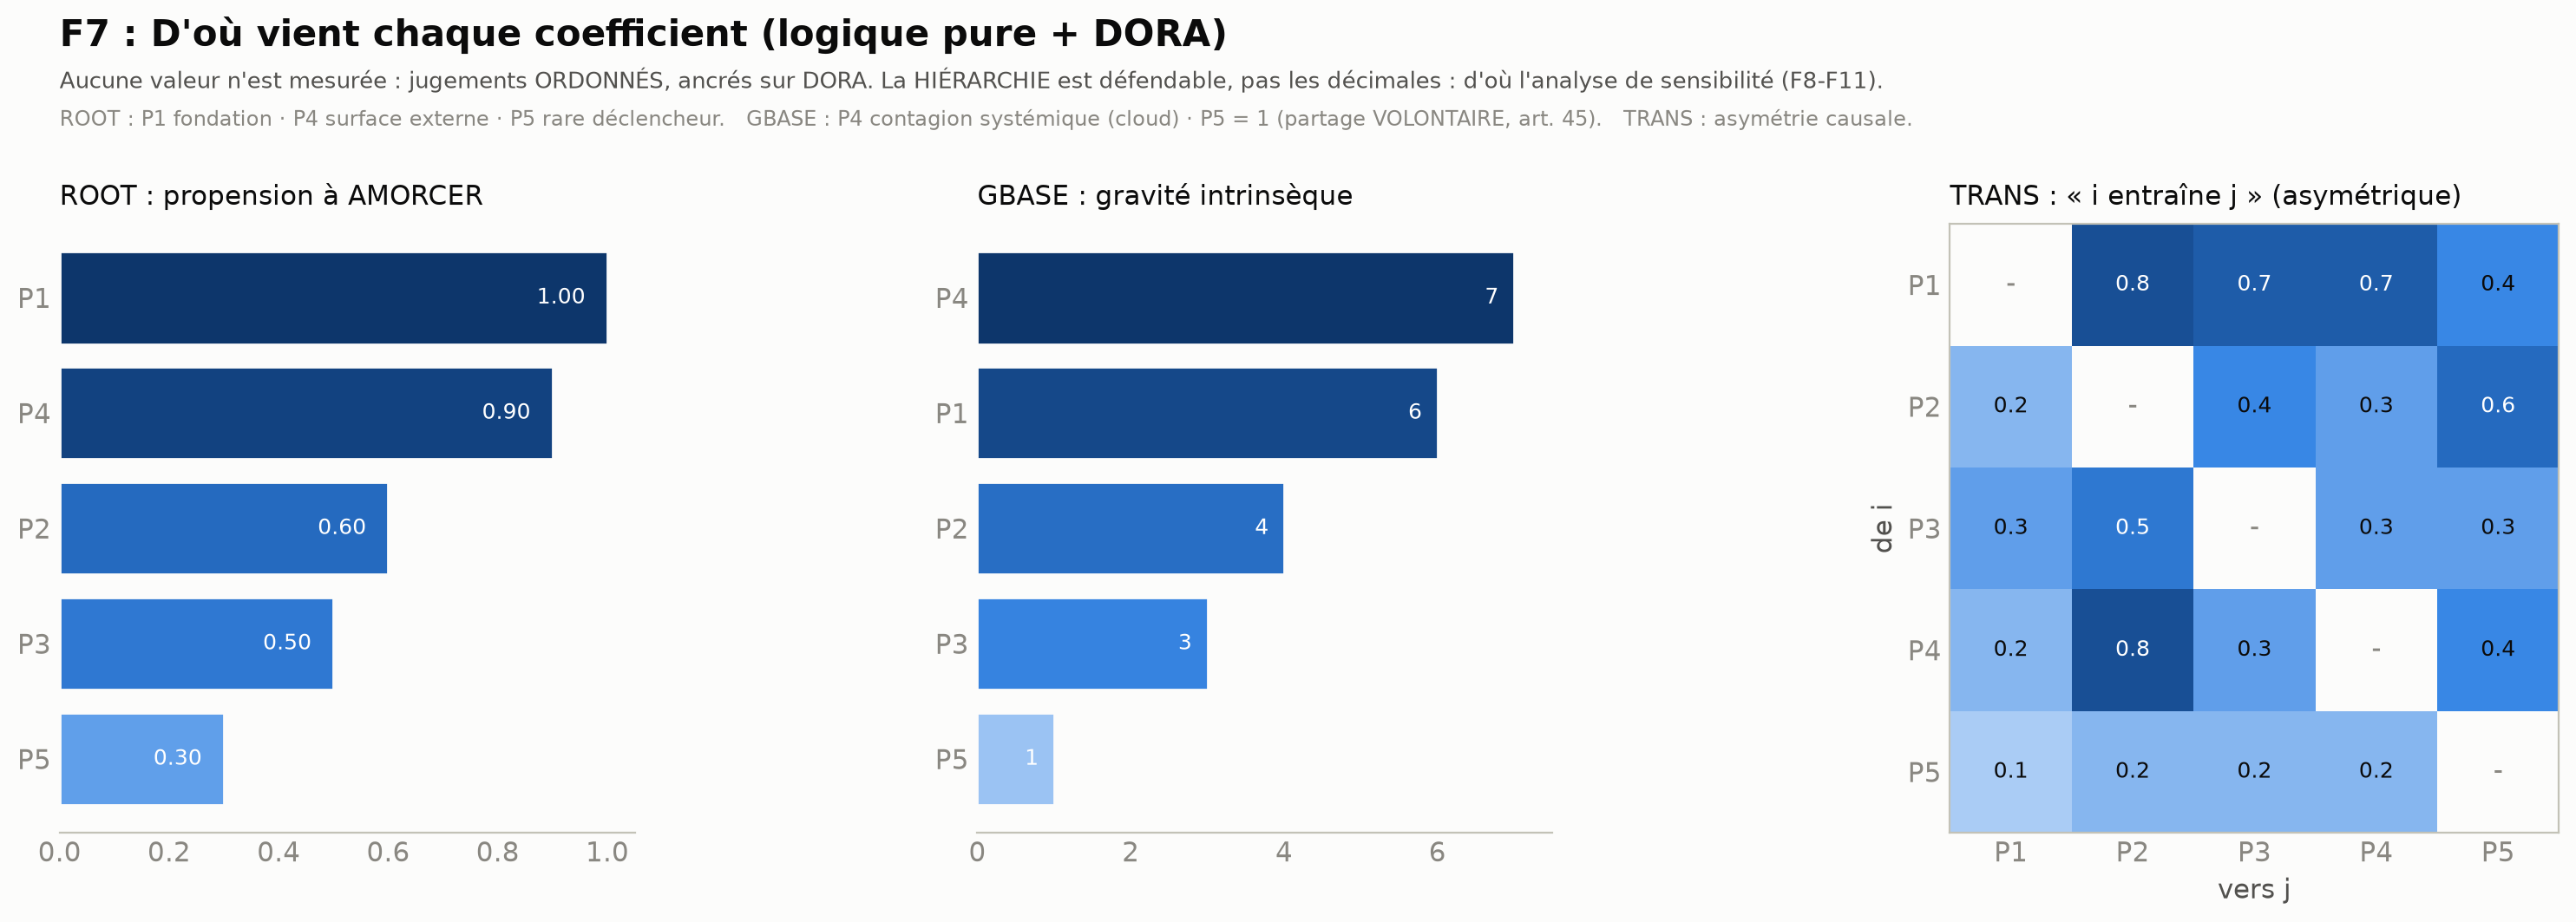
\includegraphics[width=\linewidth]{figures/F7_coefficients_ancrage.png}
\caption{D'où vient chaque coefficient : hiérarchie ordonnée, ancrée sur la structure de DORA.}
\end{figure}

\section{Robustesse : ce qui tient, ce qui ne tient pas}
\label{sec:sensi}

On ne nie pas que \og{}tout dépend des valeurs\fg{} : on le \textbf{teste}. On perturbe tous les
coefficients autour de leur base sur \textbf{3\,000 tirages} Monte-Carlo et on regarde si
les \emph{conclusions} survivent. C'est une \textbf{analyse de sensibilité globale}, où l'on
neutralise une hypothèse à la fois pour mesurer ce qu'elle porte~\cite{Saltelli2008}.

\begin{table}[h]\centering\small
\renewcommand{\arraystretch}{1.25}
\begin{tabular}{@{}p{7.2cm} l p{5.2cm}@{}}
\toprule
\textbf{Conclusion} & \textbf{Statut} & \textbf{Résultat} \\
\midrule
L'ordre renverse le verdict & \textcolor{navy}{\textbf{robuste}} & $91\%$ des paires en moyenne ; jamais $<80\%$ (100~\% des tirages) \\
Classement des pires cascades & \textcolor{navy}{\textbf{robuste}} & un scénario du Top-15 y reste dans $84\%$ des tirages \\
Plafond \og{}jamais Extrême\fg{} & \textcolor{accent}{\textbf{fragile}} & franchi dans $55\%$ des tirages $\Rightarrow$ propriété du calage, à ne pas sur-vendre \\
\bottomrule
\end{tabular}
\caption{La distinction essentielle : deux conclusions robustes, une fragile.}
\end{table}

\paragraph{Qu'est-ce qui porte le résultat ?} En neutralisant chaque hypothèse
(coefficients rendus égaux), on mesure ce qui reste de l'effet d'ordre
(amplitude moyenne $|\Delta\text{criticité}|$ entre un ordre et son inverse) :
\[
\begin{aligned}
\underbrace{2{,}90}_{\text{modèle complet}} \;&\longrightarrow\;
\underbrace{0{,}90}_{\text{sans asymétrie TRANS}} \;;\quad
2{,}50\ (\text{sans écart ROOT}) \\
&\qquad ;\quad 2{,}30\ (\text{sans écart GBASE})\;;\quad
0{,}00\ (\text{sans les trois}).
\end{aligned}
\]

\begin{figure}[h]\centering
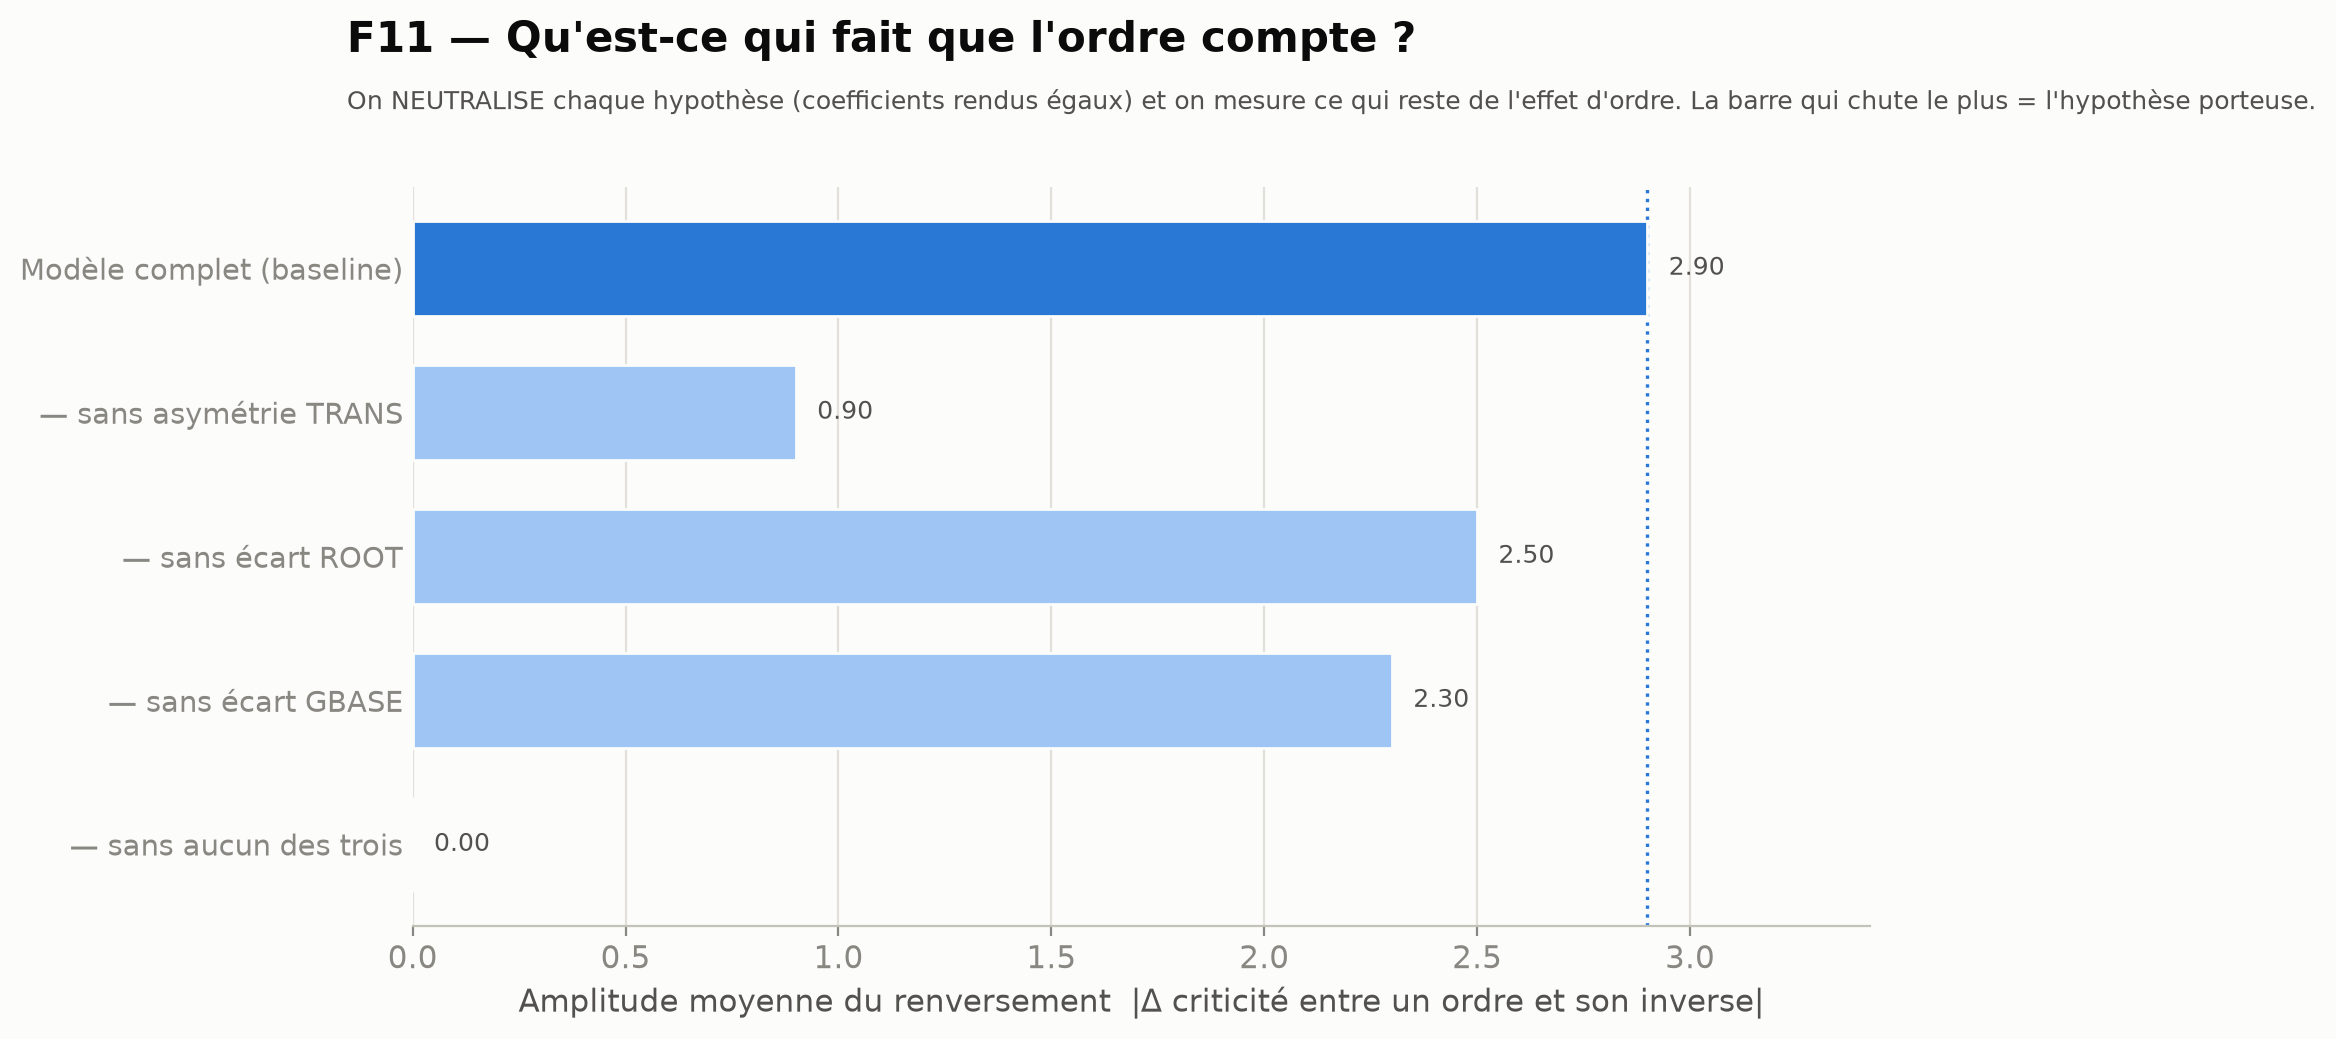
\includegraphics[width=0.82\linewidth]{figures/F11_knockout_hypotheses.png}
\caption{Neutraliser l'\textbf{asymétrie causale (TRANS)} efface l'essentiel de l'effet
($-69\%$) : c'est \emph{elle} qui porte le résultat. ROOT et GBASE ne font qu'affiner.}
\end{figure}

\begin{cle}
\textbf{Conclusion.} La seule hypothèse forte à défendre est la \textbf{direction causale
entre piliers} (TRANS asymétrique) --- l'idée qu'une attaque suit une chaîne orientée, de
l'amont vers l'aval~\cite{Hutchins2011}, et se propage de proche en proche comme une
contagion~\cite{HillairetLopez2021}. À partir d'elle, deux résultats tiennent quel que soit
le calage : \emph{l'ordre renverse le verdict} et \emph{le classement des cascades les plus
critiques}. Le plafond de criticité, lui, dépend des chiffres et n'est pas présenté comme un
résultat. Connaître et énoncer soi-même cette limite est ce qui distingue le modèle.
\end{cle}

\section{Sources des concepts mobilisés}

Le modèle qualitatif combine un socle réglementaire (DORA, Solvabilité~II) et des méthodes
établies de gestion des risques. Aucun de ces concepts n'est original~; l'apport est leur
\emph{articulation} autour de l'ordre causal. Le tableau ci-dessous relie chaque brique à sa
source.

\begin{table}[h]\centering\small
\renewcommand{\arraystretch}{1.3}
\begin{tabular}{@{}p{6.3cm} p{1.6cm} p{6.2cm}@{}}
\toprule
\textbf{Concept dans la fiche} & \textbf{Section} & \textbf{Source} \\
\midrule
Cinq piliers, gouvernance, tiers, partage volontaire & \S1 & Règlement UE 2022/2554 (DORA)~\cite{DORA2022} \\
Score \emph{criticité $=$ f(probabilité, gravité)} & \S1--2 & ISO~31000~\cite{ISO31000} ; ISO/IEC~27005~\cite{ISO27005} \\
Ne lire une matrice de risque que par son \emph{ordre} & \S1, \S4 & Cox~(2008)~\cite{Cox2008} \\
Trois barèmes = jugement d'expert structuré & \S1 & Cooke~(1991)~\cite{Cooke1991} ; O'Hagan et coll.~(2006)~\cite{OHagan2006} \\
\textbf{ROOT} = événement initiateur / n\oe{}ud-graine & \S1 & Kaplan \& Garrick~(1981)~\cite{KaplanGarrick1981} ; Kempe et coll.~(2003)~\cite{Kempe2003} \\
\textbf{TRANS} = matrice de transition / influence dirigée & \S1--2 & Pearl~(1988)~\cite{Pearl1988} ; Kempe et coll.~(2003)~\cite{Kempe2003} ; Battiston et coll.~(2012)~\cite{Battiston2012} \\
\textbf{GBASE} = axe de sévérité intrinsèque par composant & \S1 & AMDEC / IEC~60812~\cite{IEC60812} ; CVSS~\cite{CVSS} \\
Les trois barèmes ensemble = triplet du risque & \S1 & Kaplan \& Garrick~(1981)~\cite{KaplanGarrick1981} \\
Famille de méthode : RPN multiplicatif, arbres d'attaque & \S4 & IEC~60812~\cite{IEC60812} ; Schneier~(1999)~\cite{Schneier1999} ; Vesely et coll.~(1981)~\cite{Vesely1981} \\
Analogie matrice ORSA / Pilier~2 & \S4 & Directive Solvabilité~II 2009/138~\cite{SolvencyII2009} \\
Moyenne géométrique pénalisant le déséquilibre & \S2 & Grabisch et coll.~(2009)~\cite{Grabisch2009} \\
Ordre causal dirigé / chaîne d'attaque orientée & \S1--2, \S5 & Hutchins et coll.~(2011)~\cite{Hutchins2011} \\
Cascade / contagion entre composants & intro, \S5 & Hillairet \& Lopez~(2021)~\cite{HillairetLopez2021} \\
Analyse de sensibilité globale (Monte-Carlo, knockout) & \S5 & Saltelli et coll.~(2008)~\cite{Saltelli2008} \\
\bottomrule
\end{tabular}
\caption{Chaque concept et sa source. La contribution de la fiche n'est pas un concept neuf,
mais leur \emph{combinaison} autour de la direction causale entre piliers.}
\end{table}

\begin{thebibliography}{99}

\bibitem{DORA2022}
Parlement européen et Conseil de l'Union européenne.
\emph{Règlement (UE) 2022/2554 sur la résilience opérationnelle numérique du secteur
financier (DORA)}. Journal officiel de l'Union européenne, 2022.

\bibitem{SolvencyII2009}
Parlement européen et Conseil de l'Union européenne.
\emph{Directive 2009/138/CE (Solvabilité~II)}, art.~45 (ORSA). 2009.

\bibitem{ISO31000}
Organisation internationale de normalisation.
\emph{ISO 31000:2018 --- Management du risque : lignes directrices}. Genève, 2018.

\bibitem{ISO27005}
Organisation internationale de normalisation.
\emph{ISO/IEC 27005 --- Gestion des risques liés à la sécurité de l'information}. Genève.

\bibitem{Cox2008}
Cox, L.~A. Jr.
\og What's Wrong with Risk Matrices?\fg{}
\emph{Risk Analysis}, 28(2):497--512, 2008.

\bibitem{Cooke1991}
Cooke, R.~M.
\emph{Experts in Uncertainty: Opinion and Subjective Probability in Science}.
Oxford University Press, 1991.

\bibitem{OHagan2006}
O'Hagan, A., Buck, C.~E., Daneshkhah, A. et coll.
\emph{Uncertain Judgements: Eliciting Experts' Probabilities}. Wiley, 2006.

\bibitem{Grabisch2009}
Grabisch, M., Marichal, J.-L., Mesiar, R. et Pap, E.
\emph{Aggregation Functions}. Cambridge University Press, 2009.

\bibitem{Saltelli2008}
Saltelli, A., Ratto, M., Andres, T. et coll.
\emph{Global Sensitivity Analysis: The Primer}. Wiley, 2008.

\bibitem{Hutchins2011}
Hutchins, E.~M., Cloppert, M.~J. et Amin, R.~M.
\og Intelligence-Driven Computer Network Defense Informed by Analysis of Adversary
Campaigns and Intrusion Kill Chains\fg{}.
\emph{Leading Issues in Information Warfare \& Security Research}, 1:80, 2011.

\bibitem{HillairetLopez2021}
Hillairet, C. et Lopez, O.
\og Propagation of cyber incidents in an insurance portfolio\fg{}.
\emph{Scandinavian Actuarial Journal}, 2021.

\bibitem{KaplanGarrick1981}
Kaplan, S. et Garrick, B.~J.
\og On the Quantitative Definition of Risk\fg{}.
\emph{Risk Analysis}, 1(1):11--27, 1981.

\bibitem{Kempe2003}
Kempe, D., Kleinberg, J. et Tardos, {\'E}.
\og Maximizing the Spread of Influence through a Social Network\fg{}.
\emph{Proc. 9th ACM SIGKDD}, p.~137--146, 2003.

\bibitem{Pearl1988}
Pearl, J.
\emph{Probabilistic Reasoning in Intelligent Systems: Networks of Plausible Inference}.
Morgan Kaufmann, 1988.

\bibitem{Battiston2012}
Battiston, S., Puliga, M., Kaushik, R., Tasca, P. et Caldarelli, G.
\og DebtRank: Too Central to Fail? Financial Networks, the FED and Systemic Risk\fg{}.
\emph{Scientific Reports}, 2:541, 2012.

\bibitem{IEC60812}
Commission électrotechnique internationale.
\emph{IEC 60812 --- Analyse des modes de défaillance et de leurs effets (AMDEC)}. 2018.

\bibitem{CVSS}
Forum of Incident Response and Security Teams (FIRST).
\emph{Common Vulnerability Scoring System (CVSS) --- Specification Document}.

\bibitem{Schneier1999}
Schneier, B.
\og Attack Trees\fg{}.
\emph{Dr.\ Dobb's Journal}, 24(12):21--29, 1999.

\bibitem{Vesely1981}
Vesely, W.~E., Goldberg, F.~F., Roberts, N.~H. et Haasl, D.~F.
\emph{Fault Tree Handbook (NUREG-0492)}. U.S. Nuclear Regulatory Commission, 1981.

\end{thebibliography}

\end{document}
